\documentclass{article}

\usepackage[T1]{fontenc}
\usepackage{svninfo}
\usepackage{graphicx}
\usepackage[round]{natbib}
\usepackage{verbatim}
\usepackage{caption}
\usepackage{subcaption}
\usepackage{times}

\begin{document}

\bibliographystyle{abbrvnat}

\svnInfo $Id$

\newcommand{\dbatversion}{0.2}

\title{The Damped Bundle Adjustment Toolbox\\v\dbatversion{} for Matlab}
\author{Niclas B{\"o}rlin\\Department of Computing Science\\Ume{\aa}
  University\\niclas.borlin@cs.umu.se}
\date{\today}

\maketitle

\newpage

\tableofcontents

\newpage

\section{Introduction}

\subsection{Purpose}

Matlab toolbox with freely available code for bundle adjustment.
Intention to be state-of-the-art.

\subsection{Limitations}

What it can do.

What it cannot do.

\subsection{Legal}



\subsection{Scientific publications}

Refer to any of the papers...

\citet{Borlin2013:Bundle}
\citet{Borlin2013:Experiments}

\section{Installation}
\label{sec:install}

\begin{enumerate}
\item Download the package file {\tt
  \verb+dbat_+\dbatversion\verb+.zip+}.
\item Unpack the package into a directory \emph{dbat}.
\item \label{step:dbatInit}
Inside Matlab, do the following initialization:\\
\verb+cd dbat % the directory where you installed the files.+\\
\verb+dbatSetup % set paths, etc.+
\item Test the installation by executing \texttt{loadplotdemo}.
\item If \texttt{loadplotdemo} runs without errors and generates a
  figure with a camera network, the installation is ok.
\end{enumerate}

\section{Usage}

\subsection{Demos}

\subsubsection{loadplotdemo}

The \verb+loadplotdemo+ demo loads a modified Photomodeler text export
file of the 60-camera, 26000-point project used
in~\citet{Borlin2013:Bundle}. The camera network, as computed by
Photomodeler, is plotted with camera 1 aligned to the cardinal axes.
The result should look like Figure~\ref{fig:roma}. The figure is a
standard Matlab 3D figure and may e.g.\ be rotated or zoomed using the
camera toolbar.

\begin{figure*}
  \centering
  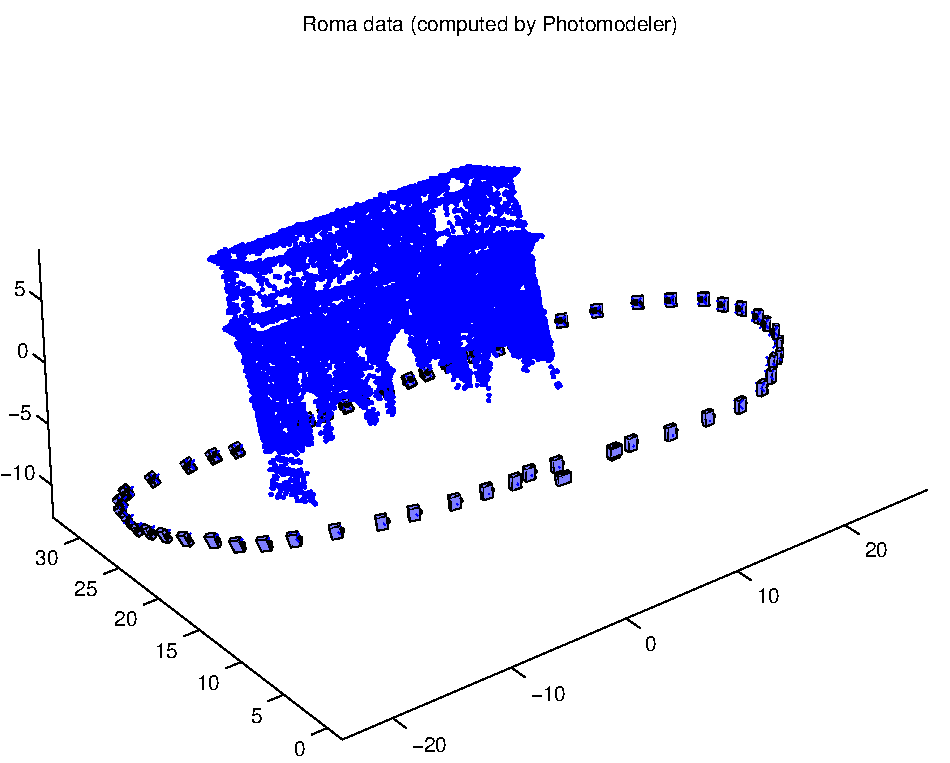
\includegraphics[width=0.6\hsize]{ill/roma}
  \caption{The figure generated by the \texttt{loadplotdemo} demo.}
  \label{fig:roma}
\end{figure*}

\subsubsection{loadplotdemo2}
\label{sec:camcaldata}

The \verb+loadplotdemo2+ demo loads a modified Photomodeler text
export file of a 21-camera, 100-point camera calibration project. The
camera network, as computed by Photomodeler, is plotted and should
look like Figure~\ref{fig:camcalib}. The figure is a standard Matlab
3D figure and may e.g.\ be rotated or zoomed using the camera toolbar.

\begin{figure*}
  \centering
  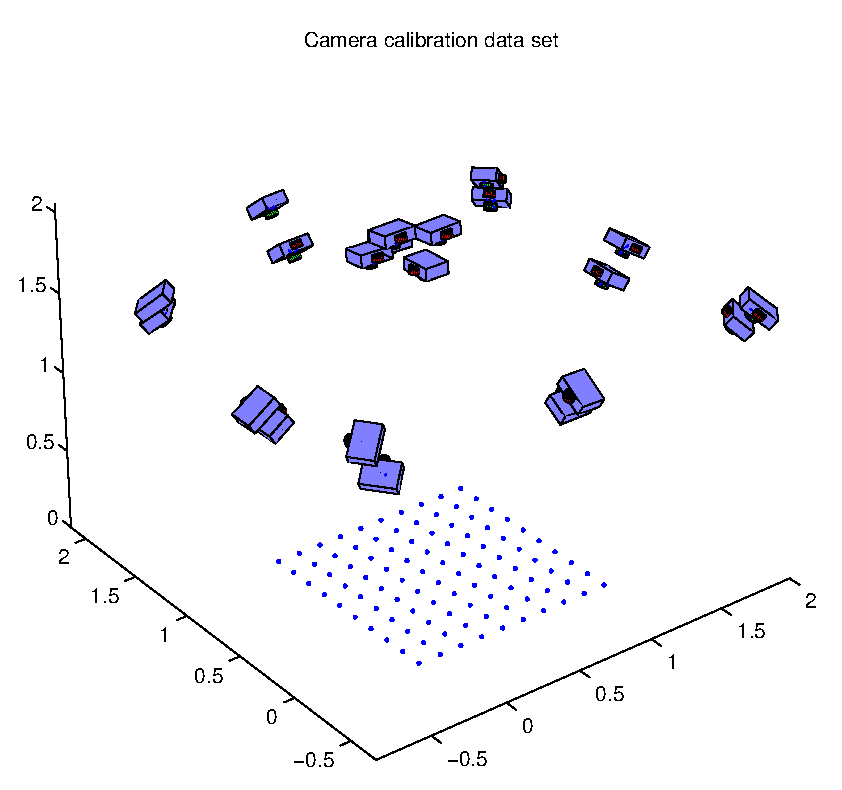
\includegraphics[width=0.6\hsize]{ill/ccam}
  \caption{The figure generated by the \texttt{loadplotdemo2} demo.}
  \label{fig:camcalib}
\end{figure*}

\subsubsection{camcaldemo}

The \verb+camcaldemo+ demo loads the camera calibration export file
from Section~\ref{sec:camcaldata} and runs a camera calibration. The
EXIF focal length is used as the initial value. The other values are
set to ``default'' values, e.g.\ the principal point at the center of
the sensor and all lens distortion parameters equal to zero. The
initial value for the EO parameters are computed by spatial
resection~\citep[Chap.~11.1.3.4]{Haralick1994:Review,McGlone2004:Manual} using
the control points defined for the Photomodeler calibration sheet. The
initial OP coordinates are subsequently computed by forward
intersection.

The bundle adjustment is run with Gauss-Newton-Armijo damping. The
result is given in a number of plot windows and a Photomodeler-style
result text file. The result plots are of two kinds: Plots that show
the evolution of the iterations and plots that show the quality of the
input or output data. The former plots may be useful to understand how
the bundle adjustment works but also to ``debug'' a difficult network
that has convergence difficulties. The latter plots give information
about the quality of the result and may also provide clues on how to
improve a network when the bundle did converge.

\paragraph{Evolution plots}

\begin{figure*}
  \centering
  \begin{subfigure}[b]{0.49\textwidth}
    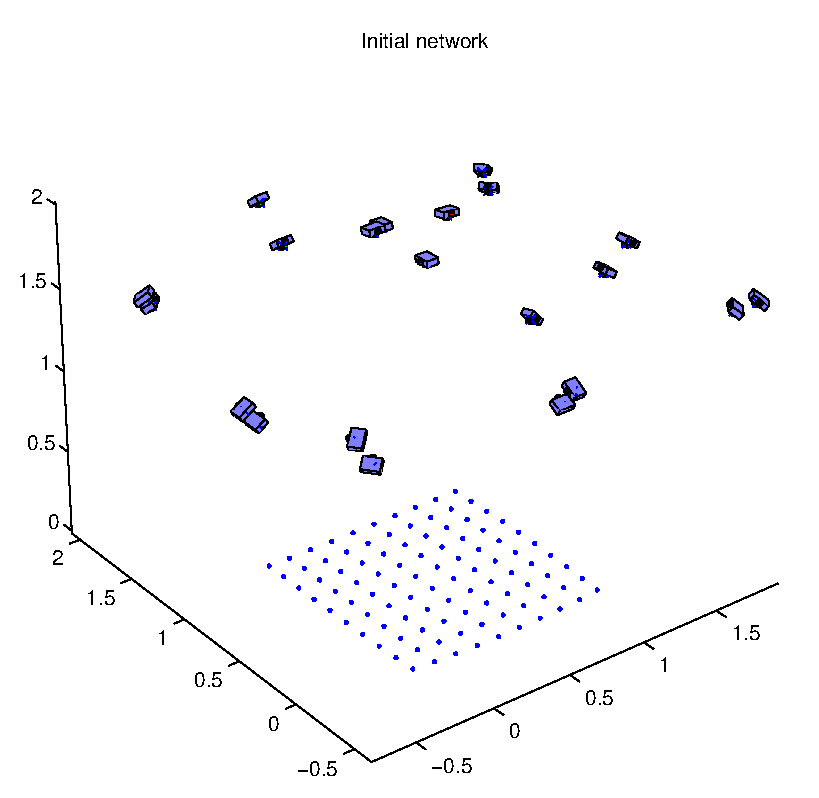
\includegraphics[width=\textwidth]{ill/ccamx0}
    \caption{Initial network configuration.\\~}
    \label{fig:camx0}
  \end{subfigure}%
  \begin{subfigure}[b]{0.49\textwidth}
    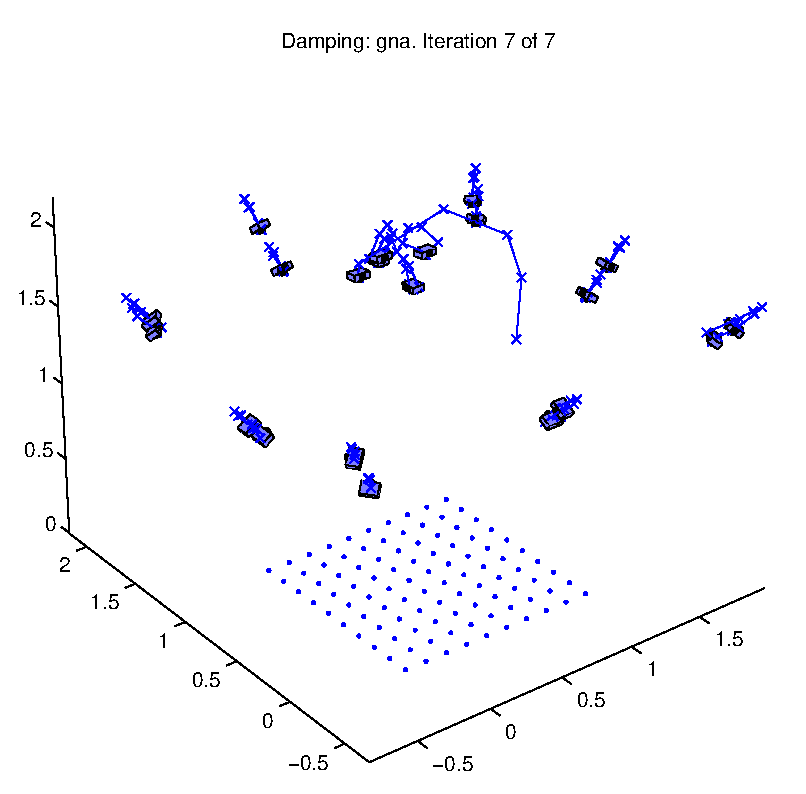
\includegraphics[width=\textwidth]{ill/ccamxfinal}
    \caption{Network configuration after convergence, with camera
      center trace lines.}
    \label{fig:camxfinal}
  \end{subfigure}
  \caption{3D network evolution during the iterations. Only the EO and
    OP parameters are illustrated. In this example, the variation of
    the OP coordinates is barely visible. }\label{fig:net3DTrace}
\end{figure*}

The evolution plots are collected in
figures~\ref{fig:net3DTrace}--\ref{fig:gnatrace}.
Figure~\ref{fig:net3DTrace} shows a snapshot of the 3D trace figure at
the beginning and end of the iterations. As default, the evolution is
presented iteration by iteration with intervening presses of the
return key. The figure window is interactive and may be rotated,
zoomed, etc. In this example, it is clear in
Figure~\ref{fig:camxfinal} that one camera station had poorer initial
values than the rest.

\begin{figure*}
  \centering
  \begin{subfigure}[b]{0.3\textwidth}
    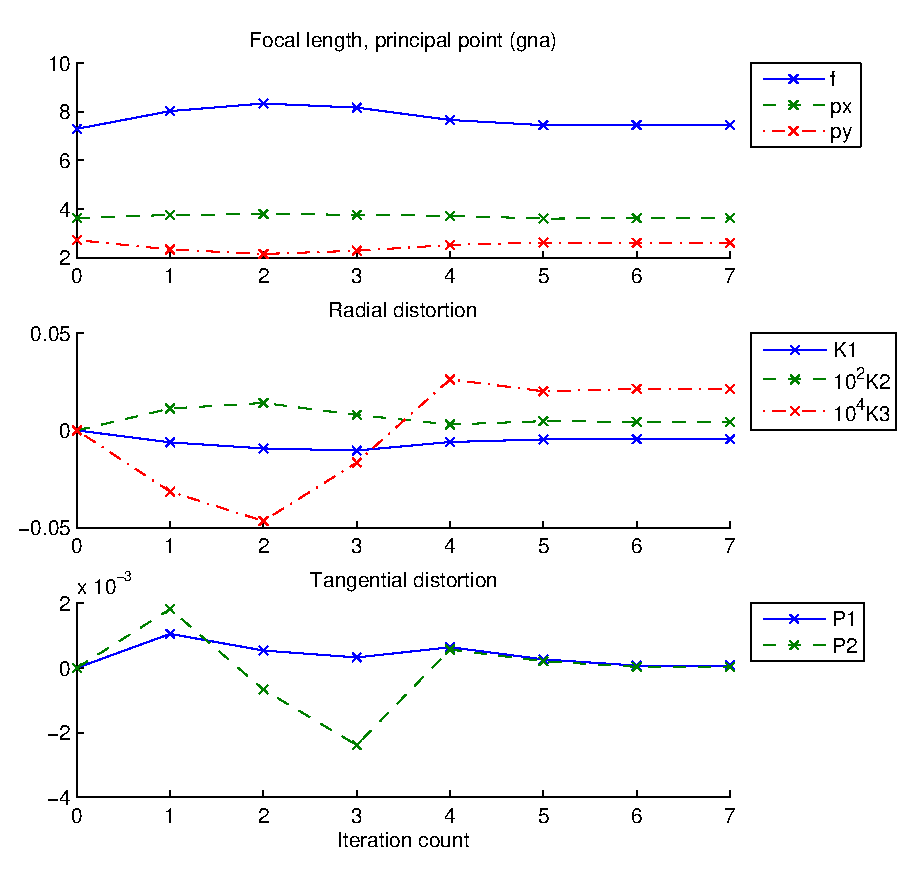
\includegraphics[width=\textwidth]{ill/ccamiotrace}
    \caption{IO parameters}
    \label{fig:IOtrace}
  \end{subfigure}%
  \begin{subfigure}[b]{0.3\textwidth}
    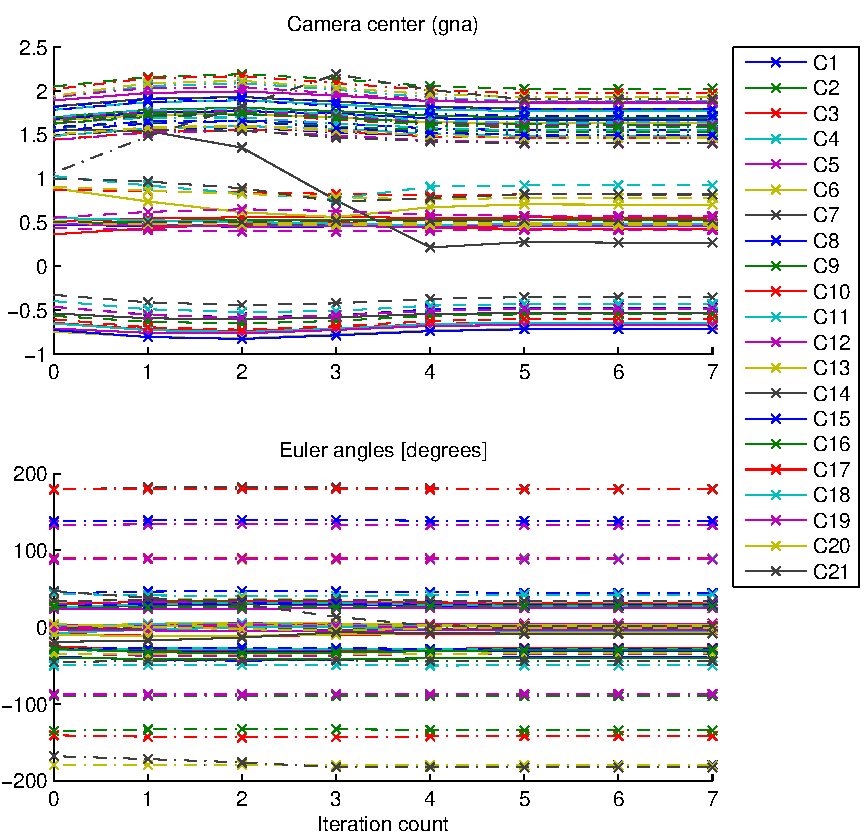
\includegraphics[width=\textwidth]{ill/ccameotrace}
    \caption{EO parameters}
    \label{fig:EOtrace}
  \end{subfigure}
  \begin{subfigure}[b]{0.3\textwidth}
    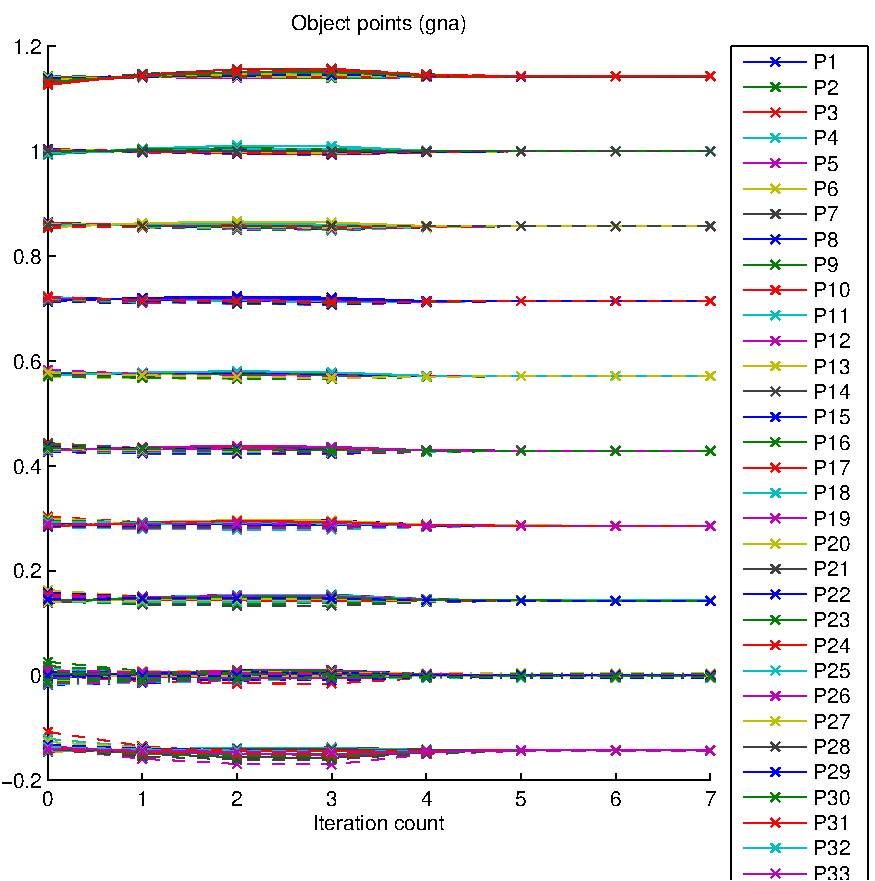
\includegraphics[width=\textwidth]{ill/ccamoptrace}
    \caption{OP parameters}
    \label{fig:OPtrace}
  \end{subfigure}
  \caption{Evolution of network parameters during the iteration
    sequence.}\label{fig:netTrace}
\end{figure*}

Figure~\ref{fig:netTrace} contains three plots showing the evolution
of the internal orientation (IO), external orientation (EO), and
object point (OP), respectively, during the iterations. The IO plot is
split into a focal/principal point panel and a radial and tangential
distortion panel, where the radial distortion parameters are scaled to
provide more information. The EO plot contains a camera center panel
and an $\omega$-$\phi$-$\kappa$ Euler angle panel. The EO and OP plots
are interactive. Lines in the plots or legends may be selected and all
corresponding lines will be highlighted. In the top panel of
Figure~\ref{fig:EOtrace}, the motion of one camera stands out.
Clicking that line reveals that it belongs to camera station~21, which
can be further investigated to decide if it should be excluded from
the calibration.

\begin{figure*}
  \centering
  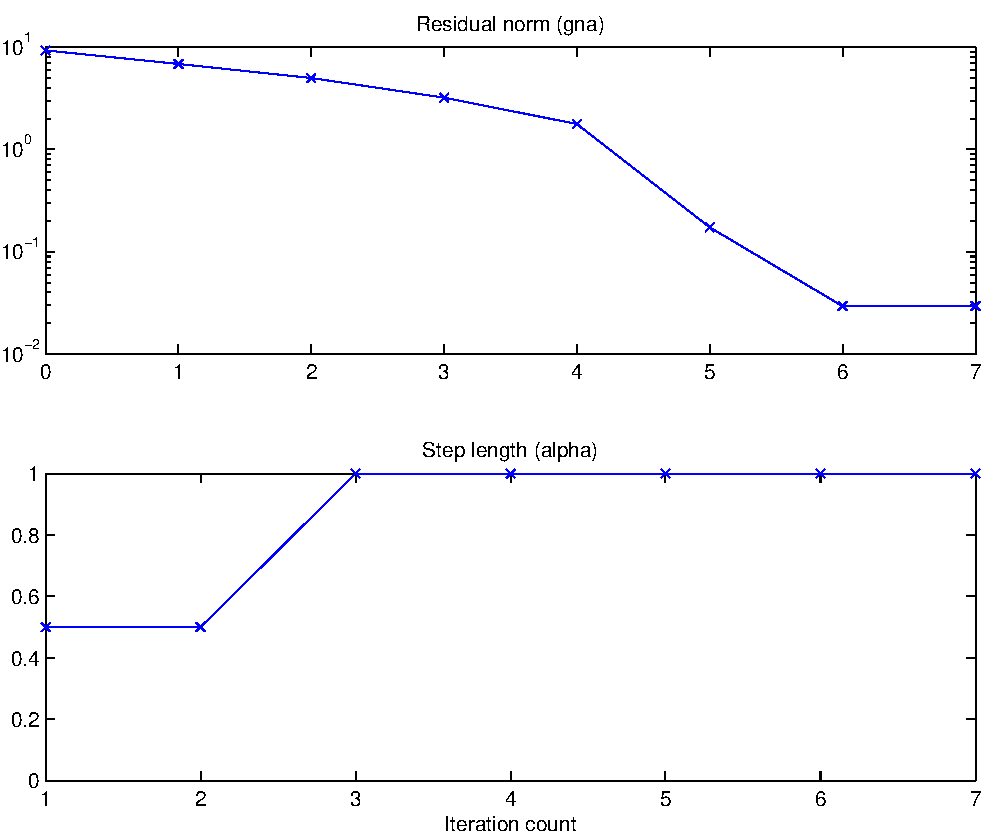
\includegraphics[width=0.5\textwidth]{ill/ccamgnatrace}
  \caption{Residual evolution and damping behaviour during the
    iterations.}
  \label{fig:gnatrace}
\end{figure*}

The final evolution plot, shown in Figure~\ref{fig:gnatrace},
illustrates the evolution of the norm of the total residual and the
damping behaviour, if any, during the bundle iterations. In this
example, the Gauss-Newton-Armijo linesearch damping is active during
the first two iterations. For further details on the damping,
see~\citet{Borlin2013:Bundle}.

\paragraph{Quality plots}

\begin{figure*}
  \centering
  \begin{subfigure}[b]{0.3\textwidth}
    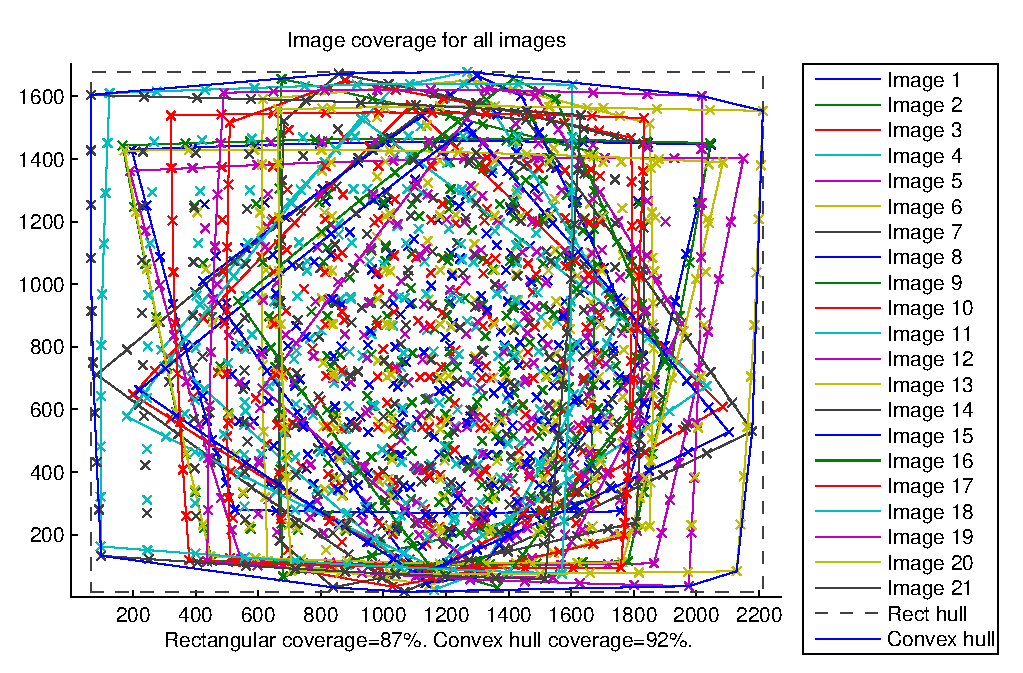
\includegraphics[width=\textwidth]{ill/ccamcoverage}
    \caption{Image coverage}
    \label{fig:ccamCoverage}
  \end{subfigure}%
  \begin{subfigure}[b]{0.3\textwidth}
    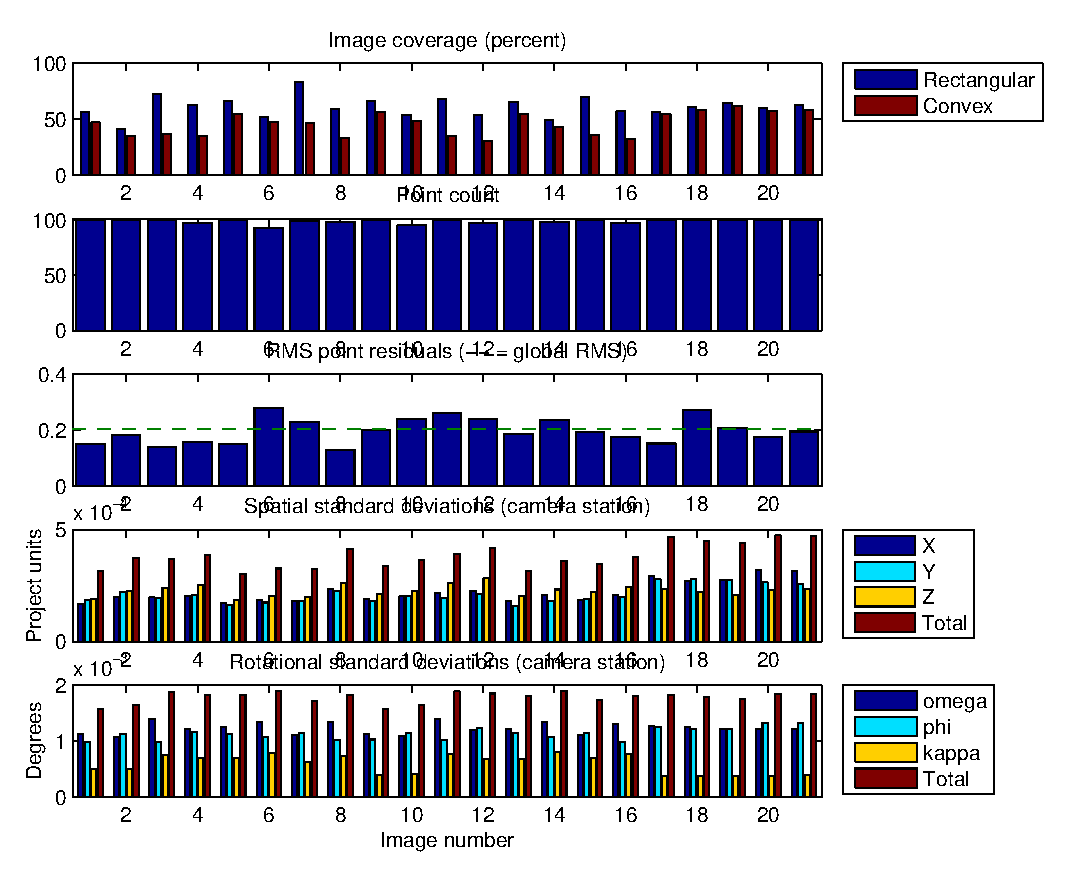
\includegraphics[width=\textwidth]{ill/ccamimstats}
    \caption{Image statistics}
    \label{fig:ccamImstats}
  \end{subfigure}
  \begin{subfigure}[b]{0.3\textwidth}
    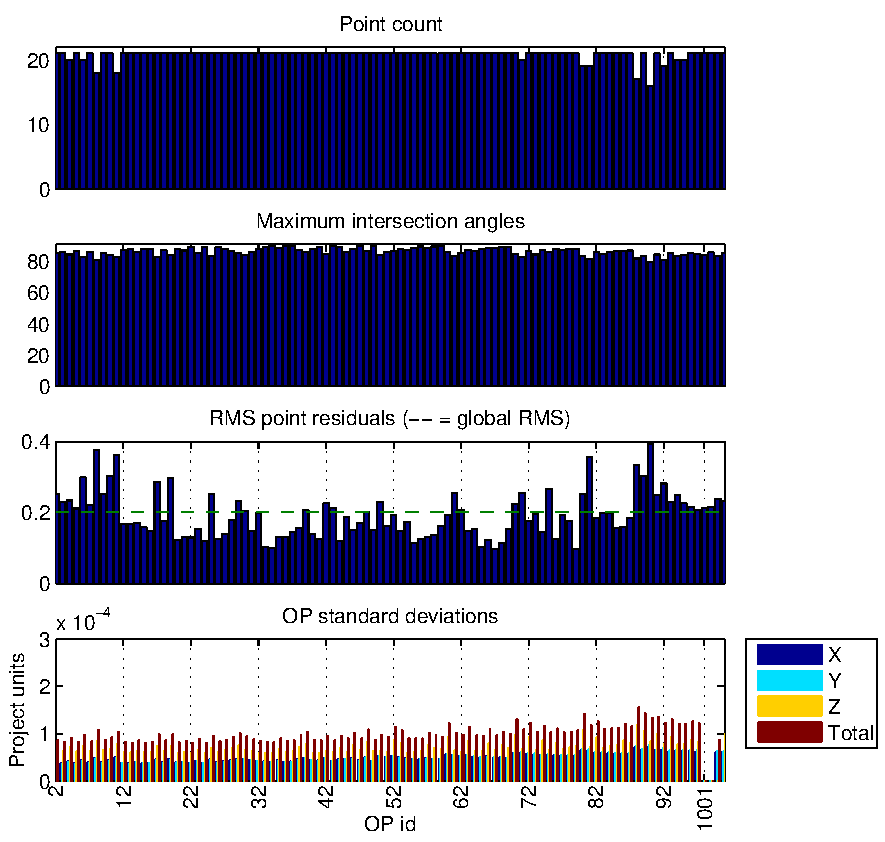
\includegraphics[width=\textwidth]{ill/ccamopstats}
    \caption{Object point statistics}
    \label{fig:ccamOPstats}
  \end{subfigure}
  \caption{Plots of input/output statistics.}\label{fig:ccamQuality}
\end{figure*}

The quality plots a gathered in Figure~\ref{fig:ccamQuality}.
Per-image quality statistics is shown in Figure~\ref{fig:ccamImstats}.
The statistics presented for each image are the image coverage; the
number of measured points; the average (RMS) point residual; and the
standard deviations for the EO parameters for the camera stations. In
this example, the data does not give any obvious support to exclude
the suspected image~21 from the calibration.

The image coverage is detailed in a separate
Figure~\ref{fig:ccamCoverage}. The plotted data is selectable. All
observations from a specific image, including their convex hull, will
be highlighted when a point or line is selected.

Finally, the per-OP quality statistics in Figure~\ref{fig:ccamOPstats}
show the number of observations per OP; the maximum ray intersection
angle; the average (RMS) point residual; and the OP coordinate
standard deviation. The presentation may be zoomed to show only a
subset of the OPs by activating the ``zoom'' function of the figure
window.

\paragraph{Result file}

The result file is modelled after the Photomodeler result file.
The result file is listed in Appendix~\ref{sec:resultFile}.

\subsubsection{romabundledemo}

\newpage
\subsection{Using your own data}

\subsubsection{Enabling text export from Photomodeler}
\label{sec:enableTextExport}.

Some versions of Photomodeler do not have the text file export option
enabled by default. In that case, follow the following steps to enable
it:
\begin{enumerate}
\item Right-click on the main window toolbar, select \emph{Customize toolbar...}.
\item In the \emph{Commands} tab, select the \emph{File} category.
\item Drag the \emph{Export Text File...} command to a toolbar of
  your choice.
\item Now you should be able to export your project as a text file by
  clicking on the \emph{Export Text File} button.
\end{enumerate}

\subsubsection{Export from Photomodeler}

To import a Photomodeler project into the toolbox, the following
steps are valid in Photomodeler Scanner 2012:

\begin{enumerate}
\item Export the project using \emph{Export Text File}. If the
  \emph{Export Text File} command is not available, follow the
  instructions in Section~\ref{sec:enableTextExport}.
\item After export, open the \emph{Project/Cameras...} dialog and
  select the camera that was used in your project.
\item Open the generated text file in a text editor.
  \begin{enumerate}
  \item On the 2nd line (usually reading \texttt{0.00005 20}), append
    the width and height in pixels of your images, e.g. to
    \texttt{0.000500 20 5616 3744}.
  \item Inspect the 4th line. For instance,
    the original data in \texttt{roma.txt} was (some trailing zeros removed):

    \texttt{24.3581 18.1143 12.0 35.96404 24.0 0.00022 -0.0 0.0 0.0 0.0}

    The values correspond to the following camera parameters:

    \texttt{focal pp\_x pp\_y format\_w format\_h K1 K2 K3 P1 P2}.

    Notice that most of the significant digits of K1--K3 were lost in
    the text export.
  \item Update the parameter values on the 4th line with values from
    the camera dialog \emph{for each parameter with a larger number of
      significant digits in the dialog}. This usually means all
    parameters except \texttt{format\_w}. In the \texttt{roma.txt}
    test case, the 4th line was modified to:

    \texttt{24.3581 18.1143 12 35.96404 24 2.174e-4 -1.518e-7 0 0 0}.

  \end{enumerate}
\end{enumerate}

\subsubsection{Loading into Matlab}

\begin{enumerate}
\item In matlab, run step~\ref{step:dbatInit} from
  Section~\ref{sec:install} if not already done.
\item \sloppy Set the variable \texttt{fName} to the text export file name \texttt{fName='c:/path/to/exported/file.txt';}, or
  select it using \texttt{[f,p]=uigetfile('*.txt'); fName=[f,p];}
\item Run the \texttt{loadplotdemo} script. A figure with your camera
  network, aligned with the first camera and rotated to have +Z 'up',
  should now have been generated.
\end{enumerate}

\bibliography{ref}

\appendix

\newpage

\section{Camera model}

\newpage

\section{Result file example}
\label{sec:resultFile}

\scriptsize
\verbatiminput{ill/C4040Z-2272x1704_result_file.txt}

\end{document}
